% xelatex
\documentclass[12pt]{article}

\usepackage{polyglossia}
\usepackage{pgfplots}
\setmainlanguage{czech}

\usepackage{graphicx, xevlna, minted} %graphics files inclusion
\usepackage{url}
\usepackage{hyperref}
\usepackage[style=iso-numeric]{biblatex}

\usepackage{hyperref}
\hypersetup{
    colorlinks=true,
    linkcolor=blue,
    filecolor=magenta,      
    urlcolor=cyan,
}

\title{
\includegraphics[width=8cm]{cvut-logo-bw.pdf}\\\vspace{2cm}NI-KOP \\ Experimentální hodnocení kvality algoritmů}
\author{\small Petr Pondělík} %doplňte své jméno, jméno vedoucího a svůj studijní obor
\date{\small Fakulta informačních technologií Českého vysokého učení technického v Praze, \\ Thákurova 9, 160 00 Praha 6 \\ \url{pondepe1@fit.cvut.cz}} %doplňte svůj email

\addbibresource{ref.bib}

\begin{document}

\maketitle              

\newpage

\section{Specifikace úlohy}

Zadání dostupné na \href{https://moodle-vyuka.cvut.cz/mod/assign/view.php?id=89700}{Moodle}.

\section{Rozbor hodnocených algoritmů}

V základu problému batohu máme zadány následující proměnné: 

\begin{itemize}
    \item celé číslo n (počet věcí)
    \item celé číslo M (kapacita batohu) 
    \item konečná množina \( V=\{v_1,v_2,…,v_n\} \) (hmotnosti věcí) 
    \item konečná množina \( C=\{c_1,c_2,…,c_n\} \) (ceny věcí)
\end{itemize}

Tato práce se zaměřuje na hodnocení algoritmů pro řešení \textbf{konstruktivní verze} optimalizačního 0/1 problému batohu.

V konstruktivní verzi optimalizačního 0/1 problému batohu hledáme množinu \( X=\{x_1,x_2,…,x_n\} \) (konfigurace) kde každé \( x_i \in \{0,1\} \) tak, aby platila nerovnost \( \sum_{i=1}^{n} x_i v_i \leq M \) (omezení) a suma \( \sum_{i=1}^{n} x_i c_i \) byla maximální (optimalizační kritérium).

\subsection{Branch\&Bound}

\subsubsection{Rozbor řešení}

Řešení problému je možné optimalizovat prořezáváním stavového prostoru. Pro dosažení rozumné optimalizace je nutné prořezávat prostor jak shora (překročení kapacity batohu), tak zdola (stávající řešení nemůže být lepší než nejlepší dosud nalezené). Asymptotická složitost řešení je stále $O(2^n)$.

\subsubsection{Postup řešení}

Ořezávání shora je implementováno testováním podmínky na aktuální hmotnost v každém rekurentním volání. Ořezávání zdola je implementováno testováním, zda v dané větvi rekurze potenciálně lze dosáhnout lepšího řešení, než je aktuální optimální řešení. Testování spočívá v přičtení sumy cen všech zbývajících předmětů k ceně aktuálního stavu a její srovnání s cenou aktuálně nejlepšího řešení.

\subsubsection{Kostra algoritmu}
\begin{listing}[ht]
    \begin{minted}[fontsize=\footnotesize]{python}
# Globálně dostupná proměnná opt (defaulně nulová cena, nekonečná hmotnost)
vyhodnotInstanci():
    zpracujStav(uroven = 1, prvni predmet nepridan, konfigurace = [])
    zpracujStav(uroven = 1, prvni predmet pridan, konfigurace = []) 
    return optimalni reseni
 
zpracujStav(uroven, stav, konfigurace): 
    konfigurace.append(stav.x)
    if stav.hmotnost > M: return
    if not potencialneLepsi(uroven, stav): return
    if uroven >= n: 
        updatujOptimum(stav, konfigurace) 
        return 
    zpracujStav(uroven++, predmet nepridan, konfigurace.add(True))
    konfigurace.pop()
    zpracujStav(uroven++, predmet pridan, konfigurace.add(False))
    konfigurace.pop()

potencialneLepsi(uroven, stav):
    ziskej zbyvajici predmety dle urovne
    pCena = stav.cena + suma cen zbyvajicich predmetu
    pHmotnost = stav.hmotnost + suma cen zbyvajicich predmetu
    return pCena > opt.cena or (pCena == opt.cena and pHmotnost < opt.hmotnost)

updatujOptimum(stav, konfigurace): 
    if (
        stav.hmotnost < M and (
            stav.cena > opt.cena or (stav.cena == opt.cena and stav.hmotnost < opt.hmotnost)
        )
    ):
        updatuj optimalni reseni aktualnim stavem a konfiguraci
    \end{minted}
\end{listing}

\newpage

\subsection{Greedy heuristika}

\subsubsection{Rozbor řešení}

Greedy heuristika staví na plnění batohu předměty v sestupném pořadí dle poměru \(\frac{cena}{hmotnost}\). Nevýhodou je, že její chyba není shora omezena.

\subsubsection{Postup řešení}

Pro instanci o vel. $n$ je definována konfigurace $\{x_1=0,...,x_n=0\}$. Předměty jsou seřazeny dle poměru \(\frac{cena}{hmotnost}\). Následně jsou iterovány a dokud řešení po zahrnutí předmětu nepřekročí kapacitu $M$, je předmět přidán do řešení. V případě přidání i-tého předmětu je v konfiguraci nastavena hodnota $x_i=1$ a cena řešení je inkrementována o jeho hmotnost.

\subsubsection{Kostra algoritmu}

\begin{listing}[ht]
    \begin{minted}[fontsize=\footnotesize]{python}
solution # Globální proměnná (defaulně nulová cena a hmotnost)
X = [0, ..., 0] # Pole o velikosti instance
for item in items:
    if solution.weight + item.weight <= M:
        solution.cost += item.cost
        solution.weight += item.weight
        X[item.inx] = 1
    \end{minted}
\end{listing}

\subsection{Dynamické programování}

\subsubsection{Rozbor řešení}

Dynamické programování (DP) využívá dekompozici instance problému. Řešení podproblémů vzniklých dekompozicí jsou ukládána do paměti a znovupoužita v případě potřeby řešit již známý podproblém. DP tedy převádí časovou složitost na složitost paměťovou.

Pro řešení problému batohu pomocí DP lze využít dekompozici dle váhy či ceny. V případě dekompozice dle ceny pak hledáme řešení inverzního problému batohu. Tedy pro daný počet předmětů n a cenu C hledáme konfiguraci \( X=\{x_1,x_2,…,x_n\} \) takovou, aby \( \sum_{i=1}^{n} x_ic_i = C \) (omezení) a suma \( \sum_{i=1}^{n} x_iw_i \) byla minimální (optimalizační kritérium).

Velikost potřebné paměti je \(n \sum_{i=1}^{n}c_i\). Každý prvek lze spočítat v konstantním čase. Nechť \(C_M = max\{c_1, c_2, ..., c_n\}\). Pak \(\sum_{i=1}^{n}c_i \leq n C_M\). Asymptotická složitost této varianty je tedy \( O(n^2 C_M) \). Parametr $C_M$ nezávisí na velikosti instance, tudíž se jedná o pseudopolynomiální algoritmus.

\subsubsection{Postup řešení}

Využita je dekompozice dle ceny. DP je vyřešeno iterativně. Alokována je tabulka \textbf{memory} hmotností (hodnoty $\infty$) o velikosti $(n+1)(C_{sum}+1)$, kde $C_{sum}=\sum_{i=1}^{n}c_{i}$. Z optimalizačního důvodu jsou ceny předmětů s hmotností přesahující M nastaveny na 0 (nižší $C_{sum}$). Definujeme $memory[0][0]=0$. Následně jsou řešeny postupně rostoucí podproblémy o $n^{'}$ prvcích z množiny $\{1,...,n\}$ plnění batohu tak, aby $\sum_{i=1}^{n^{'}} x_ic_i = C$ (omezení) a suma $\sum_{i=1}^{n^{'}} x_iw_i$ byla minimální. Opakující se podproblémy nejsou opakovaně počítány, ale je využíváno již vyřešených podproblémů. Minimální váha, pomocí které lze dosáhnout ceny $c$ pro instanci o $i+1$ prvních předmětech, je získána vztahem $memory[c][i+1] = min(memory[c][i], memory[c-c_{i+1}][i] + w_{i})$. Tedy zkoumáme, odkud jsme na aktuální pole tabulky mohli přistoupit v případě, že nový předmět nepřidáme ($memory[c][i]$), či přidáme ($memory[c-c_{i+1}][i] + w_{i}$) a vybíráme hodnotu s nižší hmotností.

Výslednou cenu $C_{res}$ nalezneme jako maximální řádkový index $c$ prvku posledního sloupce tabulky, jehož váha je $\leq M$. Konstrukce konfigurace řešení získáme pomocí backtrackingu z pozice ceny $C_{res}$. Vycházíme ze souřadnic optimálního řešení a postupně zmenšujeme řešený problém odebíráním předmětů. Pokud se při zmenšení problému nezmění minimální hmotnost (porovnání $memory[c][i] = memory[c][i-1]$), předmět nepatří do konfigurace řešení.

\newpage

\subsubsection{Kostra algoritmu}

\begin{listing}[ht]
    \begin{minted}[fontsize=\footnotesize]{python}
# Globální proměnné
n, M, C, W, cSum, solution
memory = [[inf for i in {0, ..., n+1}] for j in {0, ..., cSum+1)]
memory[0][0] = 0
for i in {1, ..., n+1}:
    for cost in C:
        memory[cost][i+1] = min(memory[cost][i], memory[cost - C[i+1]][i] + W[i])

findSolution(memory):
    return memory[c,n], kde memory[c,n] <= M a c je maximalni

findSolutionConf(memory, cost):
    conf = [0 for i in {0, ..., n}]
    actualCost, actualItem = cost, n
    for i in {1, n + 1}:
        originItem, originCost = actualItem-1, actualCost
        originWeight = self.memory[actualCost][originItem]
        actualWeight = self.memory[actualCost][actualItem]
        if actualWeight != originWeight:
            originCost = actualCost - C[n-i]
            conf[n-i] = 1
            actualCost, actualItem = originCost, originItem
    return conf

solution.cost = findSolution(memory)
solution.configuration = findSolutionConf(memory, solution.cost)

return solution

    \end{minted}
\end{listing}

\newpage

\section{Experimentální vyhodnocení}

\subsection{Specifikace platformy}

Procesor: Intel Core i5-10210U, 1.6 GHz (TurboBoost 4.2 GHz) \\
Operační systém: Kubuntu 20.04.1 LTS \\
Programovací jazyk: Python 3.8

\subsection{Generátor instancí}

Pro účely generování dat byl využit generátor instancí problému batohu dostupný na stránkách kurzu.

Popis parametrů generátoru vyskytujících se dále v textu:
\begin{itemize}
    \item -n: počet předmětů [celé číslo],
    \item -N: počet instancí [celé číslo],
    \item -m: poměr kapacity batohu k sumární váze jako pevná hodnota [reálné číslo],
    \item -W: maximální váha předmětu [celé číslo],
    \item -w: převaha lehkých/těžkých věcí [bal|light|heavy],
    \item -C: maximální cena předmětu [celé číslo],
    \item -c: korelace s váhou žádná/menší/silná [uni|corr|strong],
    \item -k: exponent granularity [reálné číslo]
\end{itemize}

\subsection{Branch \& Bound}

\subsubsection{Citlivost výp. času na poměr kapacity batohu k sumární váze}

\subsubsection*{Hypotéza} \label{section:bnb_hyp}

Předpokládejme, že pro poměr kapacity batohu k sumární váze v intervalu $[0.0, 0.5]$ bude při rostoucím poměru růst rovněž výpočetní čas. Dále předpokládejme, že pro poměr v intervalu $(0.5, 1.0]$ bude výpočetní čas klesat. Hypotéza je založena na myšlence, že pokud je poměr v intervalu $[0.0, 0.5]$, dochází s klesajícím poměrem k většímu ořezávání shora (na základě překročení kapacity batohu), resp. pokud je poměr v intervalu $(0.5, 1.0]$, dochází s rostoucím poměrem k většímu ořezávání zdola (stávající řešení nemůže být lepší než nejlepší dosud nalezené).

\subsubsection*{Příprava dat pro experimentální vyhodnocení}

Pro účely experimentálního vyhodnocení byla pro $n \in \{5, 10, 15, 20, 22\}$ vygenerována skupina datových sad s prefixem \textbf{m}.

Vlastnosti sad (dle konfigurace generátoru) jsou následující:

\begin{center}
    \begin{tabular}{|c | c | c | c | c | c | c|} 
        \hline
        -N & -m & -W & -w & -C & -c & -k \\ [0.1ex]
        \hline\hline
        500 & \{0.1, 0.2, 0.3, 0.4, 0.5, 0.6, 0.7, 0.8, 0.9\} & 300 & bal & 1500 & corr & 1\\
        \hline
    \end{tabular}
\end{center}

\subsubsection*{Výsledky měření}

Naměřené časy jsou k dispozici v tabulce \ref{tab:bnb_time_n_dep}.

Data jsou vizualizována třemi grafy. Na grafu \ref{fig:bnb_time_n_dep_1} můžeme vidět srovnání CPU časů metody B\&B v závislosti na velikosti instance n pro $m \in \{0.1, 0.2, 0.3, 0.4, 0.5\}$. Na srovnání můžeme s rostoucí hodnotou m pozorovat rostoucí CPU čas. Naopak na grafu \ref{fig:bnb_time_n_dep_2} (pro $m \in \{0.5, 0.6, 0.7, 0.8, 0.9\}$) lze pozorovat klesající CPU čas s rostoucí hodnotou m. Graf \ref{fig:bnb_time_m_dep} pak poskytuje jiný pohled na data a zachycuje vývoj CPU času pro konkrétní volby n v závislosti na m. Můžeme pozorovat, že maximální CPU čas byl naměřen při volbě $m=0.5$. S m vzdalujícím se od hodnoty $0.5$ CPU čas klesá.

Naměřené výsledky tedy potvrzují hypotézu \ref{section:bnb_hyp}.

\begin{table}
    \begin{center}
         \begin{tabular}{|c | c | c | c | c | c | c | c | c | c|} 
         \hline
         n & m=0,1 & m=0,2 & m=0,3 & m=0,4 & m=0,5 & m=0,6 & m=0,7 & m=0,8 & m=0,9 \\ [0.1ex] 
         \hline\hline
        5 & 0,01 & 0,01 & 0,01 & 0,01 & 0,01 & 0,01 & 0,01 & 0,01 & 0,01 \\
        \hline
        10 & 0,12 & 0,98 & 1,15 & 1,68 & 1,93 & 1,72 & 1,22 & 0,91 & 0,09 \\
        \hline
        15 & 1,77 & 7,50 & 19,04 & 34,05 & 40,90 & 33,24 & 18,38 & 6,64 & 1,47 \\
        \hline
        20 & 10,67 & 84,05 & 364,40 & 815,64 & 1038,87 & 757,42 & 315,44 & 69,50 & 7,27 \\
        \hline
        22 & 22,54 & 242,73 & 1258,16 & 3073,87 & 3990,42 & 2810,46 & 1048,21 & 189,55 & 13,95 \\
        \hline
        \end{tabular}
        \caption{Průměrný CPU čas B\&B dle volby m [ms]}
        \label{tab:bnb_time_n_dep}
    \end{center}
\end{table}

\begin{figure}[ht]\centering
    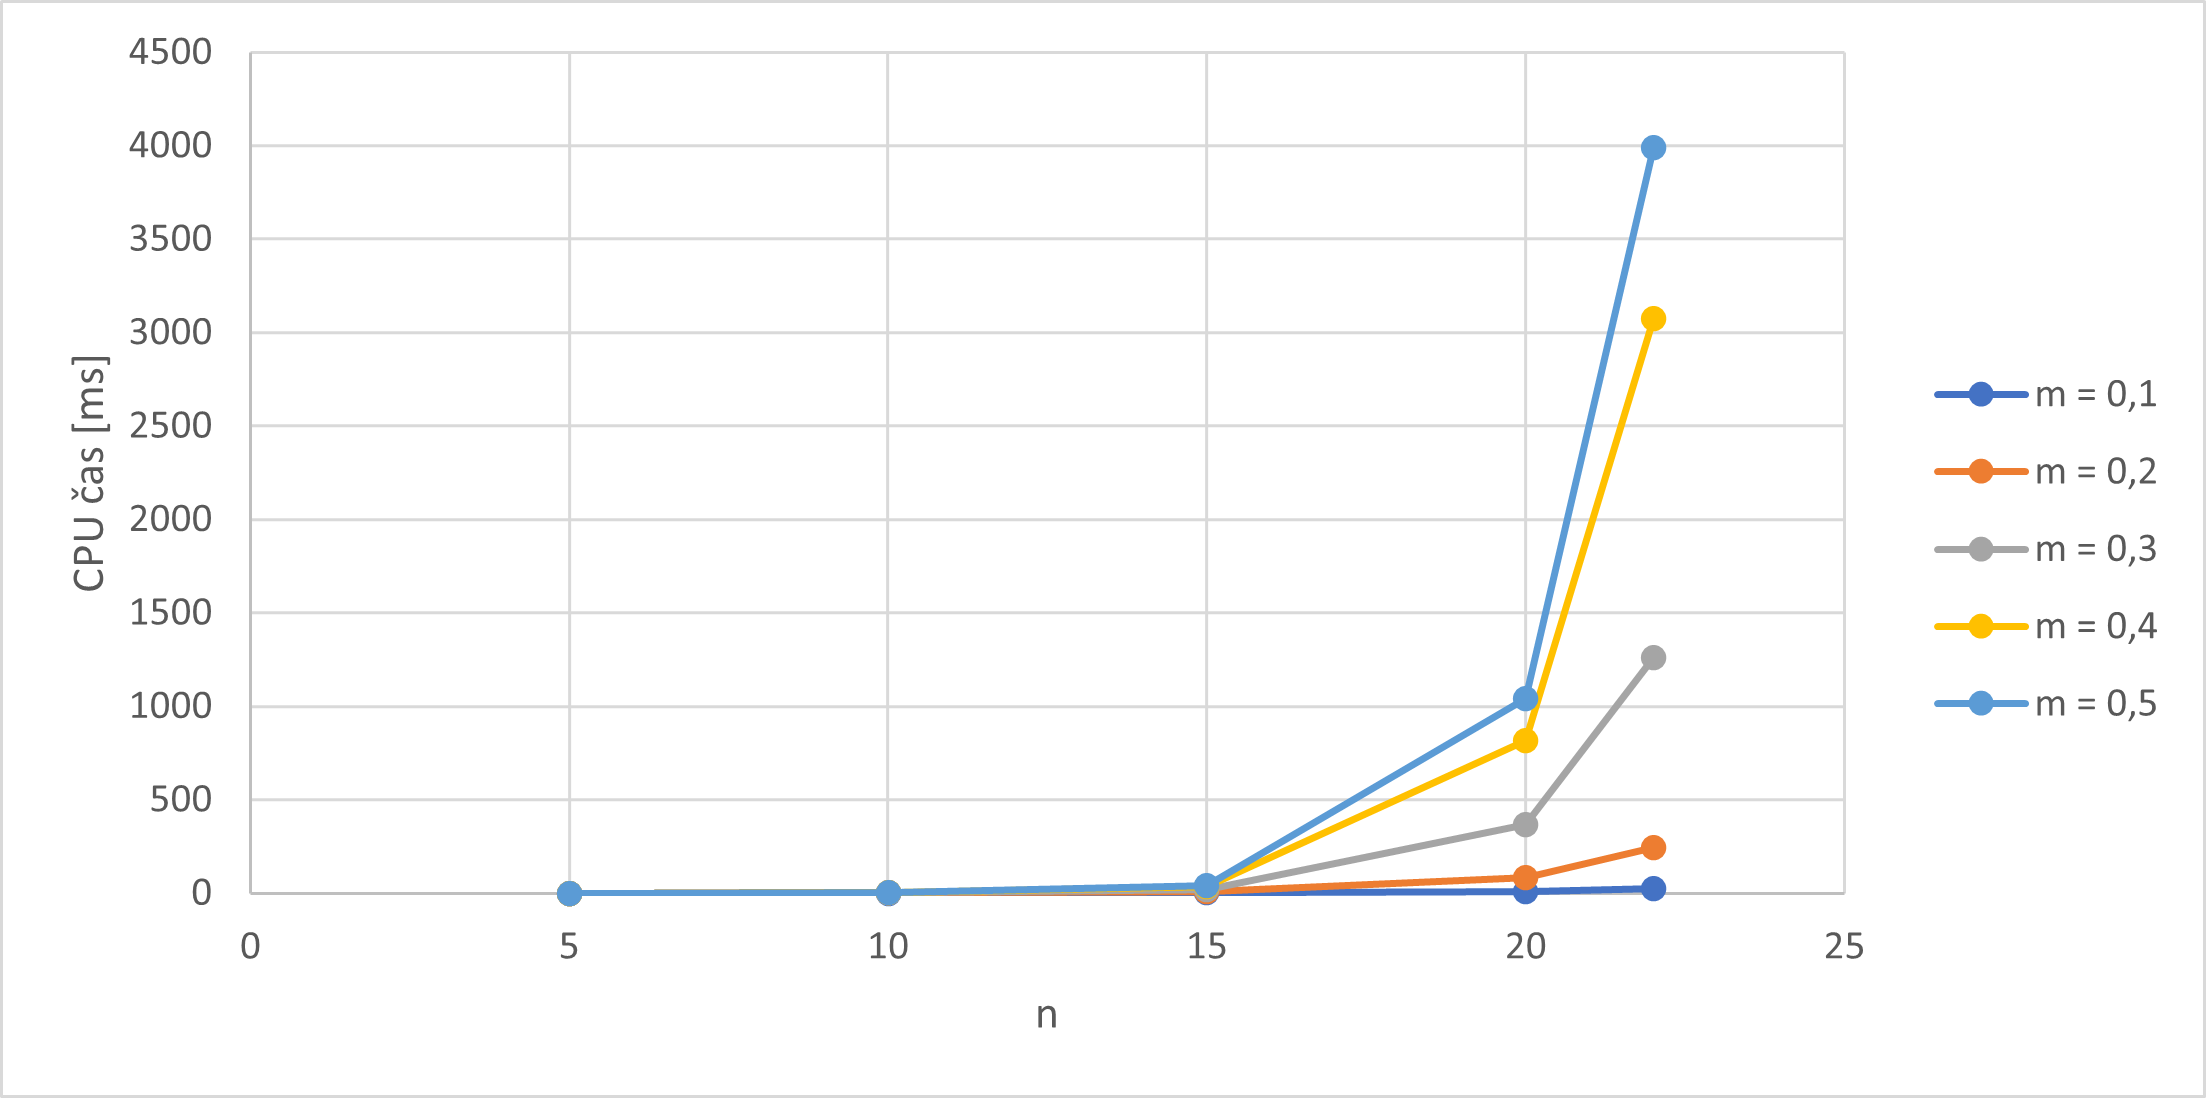
\includegraphics[width=1\textwidth, keepaspectratio]{graphs/bnb/bnb_time_n_dep_1.png}
    \caption{Závislosti CPU času B\&B na n pro parametr $m \in \{0.1, 0.2, 0.3, 0.4, 0.5\}$}
    \label{fig:bnb_time_n_dep_1}
\end{figure}

\begin{figure}[ht]\centering
    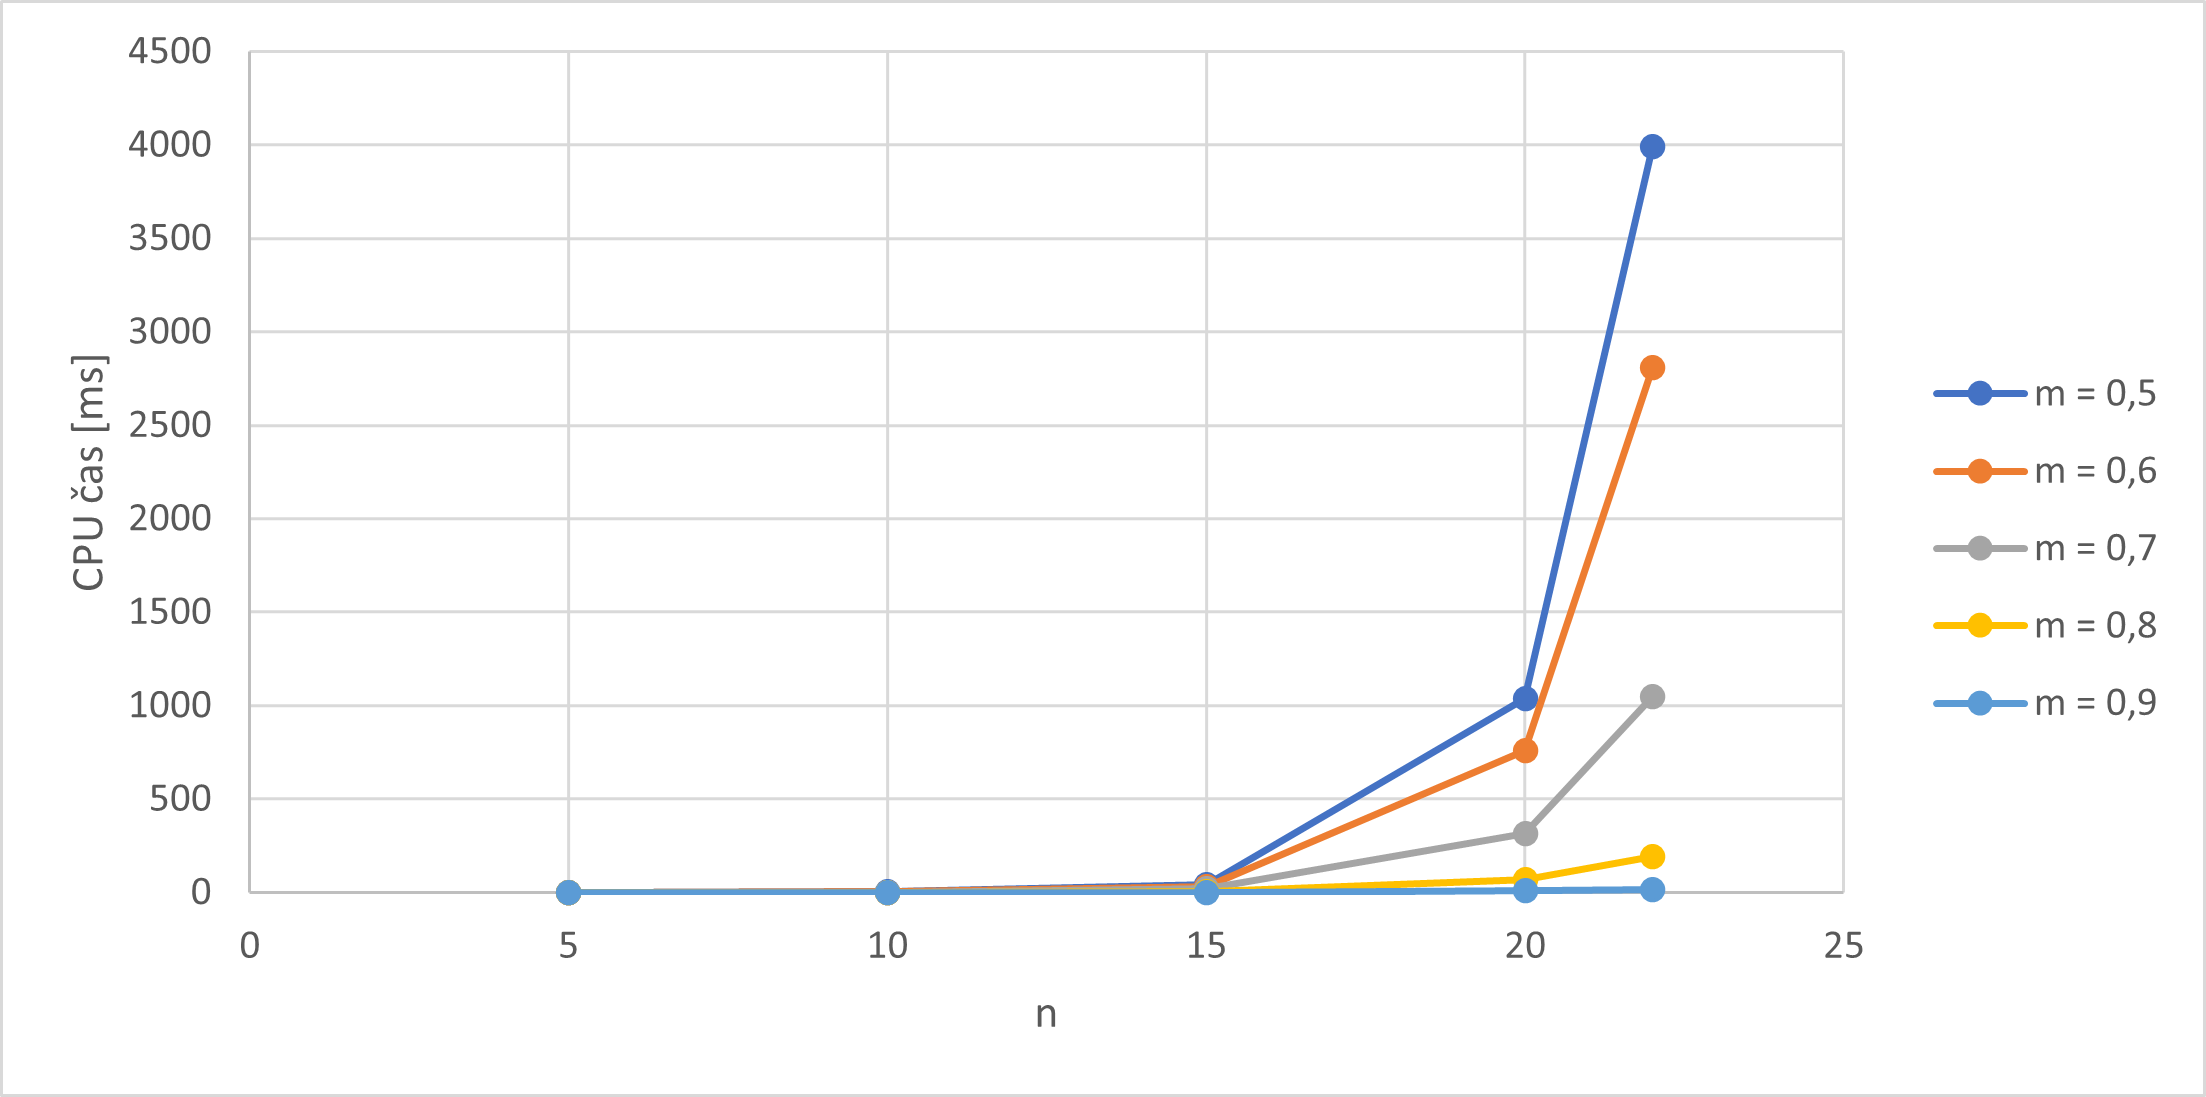
\includegraphics[width=1\textwidth, keepaspectratio]{graphs/bnb/bnb_time_n_dep_2.png}
    \caption{Závislost CPU času B\&B na n pro parametr $m \in \{0.5, 0.6, 0.7, 0.8, 0.9\}$}
    \label{fig:bnb_time_n_dep_2}
\end{figure}

\begin{figure}[ht]\centering
    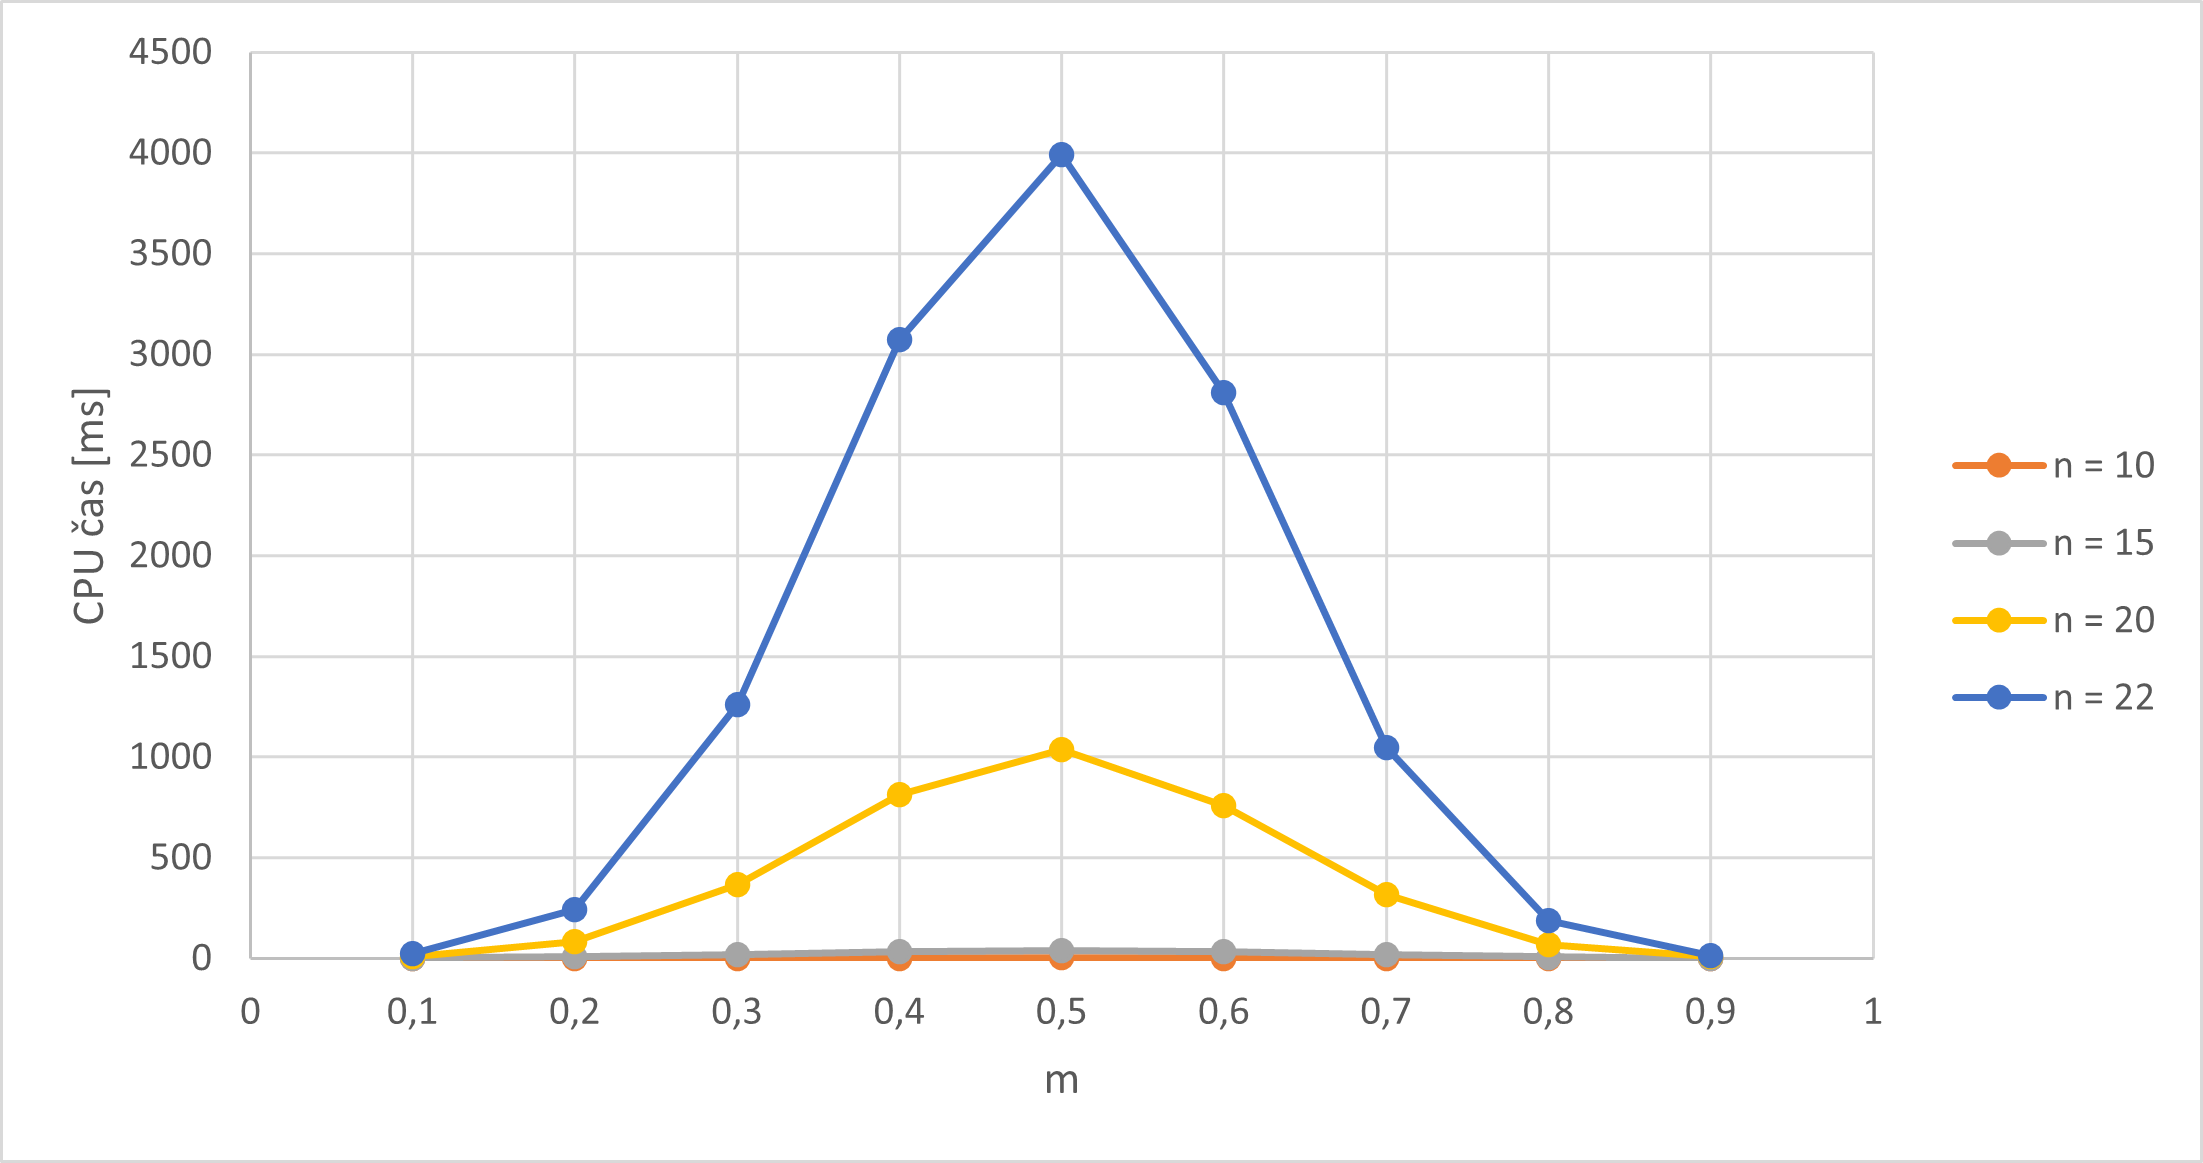
\includegraphics[width=1\textwidth, keepaspectratio]{graphs/bnb/bnb_time_m_dep.png}
    \caption{Závislosti CPU času B\&B na parametru m pro $n \in \{10, 15, 20, 22\}$}
    \label{fig:bnb_time_m_dep}
\end{figure}

\subsection{Greedy heuristika}

\subsubsection{Citlivost chyby na granularitu}

\subsubsection*{Hypotéza} \label{section:greedy_granularity_hyp}

Mějme batoh s kapacitou relativně nízkou vůči sumární váze předmětů. Dále měníme granularitu předmětů směrem dolů (tedy dostáváme stále menší předměty - předměty s nižší vahou). Předpokládejme, že chyba heuristiky bude klesat.

\subsubsection*{Příprava dat pro experimentální vyhodnocení}

Pro účely experimentálního vyhodnocení byla pro $n \in \{5, 10, 15, 20, 22, 25\}$ vygenerována skupina datových sad s prefixem \textbf{k}.
Vlastnosti sad (dle konfigurace generátoru) jsou následující:

\begin{center}
    \begin{tabular}{|c | c | c | c | c | c | c|}
        \hline
        -N & -m & -W & -w & -C & -c & -k \\ [0.1ex]
        \hline\hline
        500 & 0.2 & 300 & light & 1500 & uni & \{1, 5, 10, 50, 100, 200, 300\}\\
        \hline
    \end{tabular}
\end{center}

\subsubsection*{Výsledky měření} \label{section:greedy_granularity_res}

Naměřené průměrné chyby jsou k dispozici v tabulce \ref{tab:greedy_granularity_error}. Hodnoty chyb byly získány jakožto průměrné relativní odchylky od optimálních řešení (optimální řešení byla získána pomocí metody B\&B).

Data jsou vizualizována dvěma grafy. Na grafu \ref{fig:greedy_granularity_error_n_dep} můžeme pozorovat klesající průměrnou chybu v závislosti na velikosti instance n při rostoucím koeficientu $k$. Výrazný pokles chybovosti pak lze pozorovat pro volby $k \in \{200, 300\}$. Na grafu \ref{fig:greedy_granularity_error_k_dep} lze pozorovat klesající průměrnou chybu s rostoucí hodnotou koeficientu $k$ pro konkrétní volby $n$.

Naměřené výsledky tedy potvrzují hypotézu \ref{section:greedy_granularity_hyp}.

\begin{table}
    \begin{center}
         \begin{tabular}{|c | c | c | c | c | c | c|} 
         \hline
         n & k=1 & k=5 & k=50 & k=100 & k=200 & k=300 \\ [0.1ex] 
         \hline\hline
            5 & 2,714 & 2,332 & 2,944 & 2,467 & 0,964 & 0,307 \\
            \hline
            10 & 2,391 & 2,117 & 1,868 & 1,764 & 0,896 & 0,295 \\
            \hline
            15 & 1,432 & 1,595 & 1,277 & 1,064 & 0,460 & 0,157 \\
            \hline
            20 & 1,168 & 1,116 & 0,942 & 0,913 & 0,257 & 0,037 \\
            \hline
            22 & 1,152 & 0,951 & 0,924 & 0,649 & 0,207 & 0,087 \\
            \hline
            25 & 0,921 & 0,868 & 0,881 & 0,666 & 0,200 & 0,047 \\
            \hline
        \end{tabular}
        \caption{Průměrná chyba greedy heuristiky dle volby k [\%]}
        \label{tab:greedy_granularity_error}
    \end{center}
\end{table}

\begin{figure}[ht]\centering
    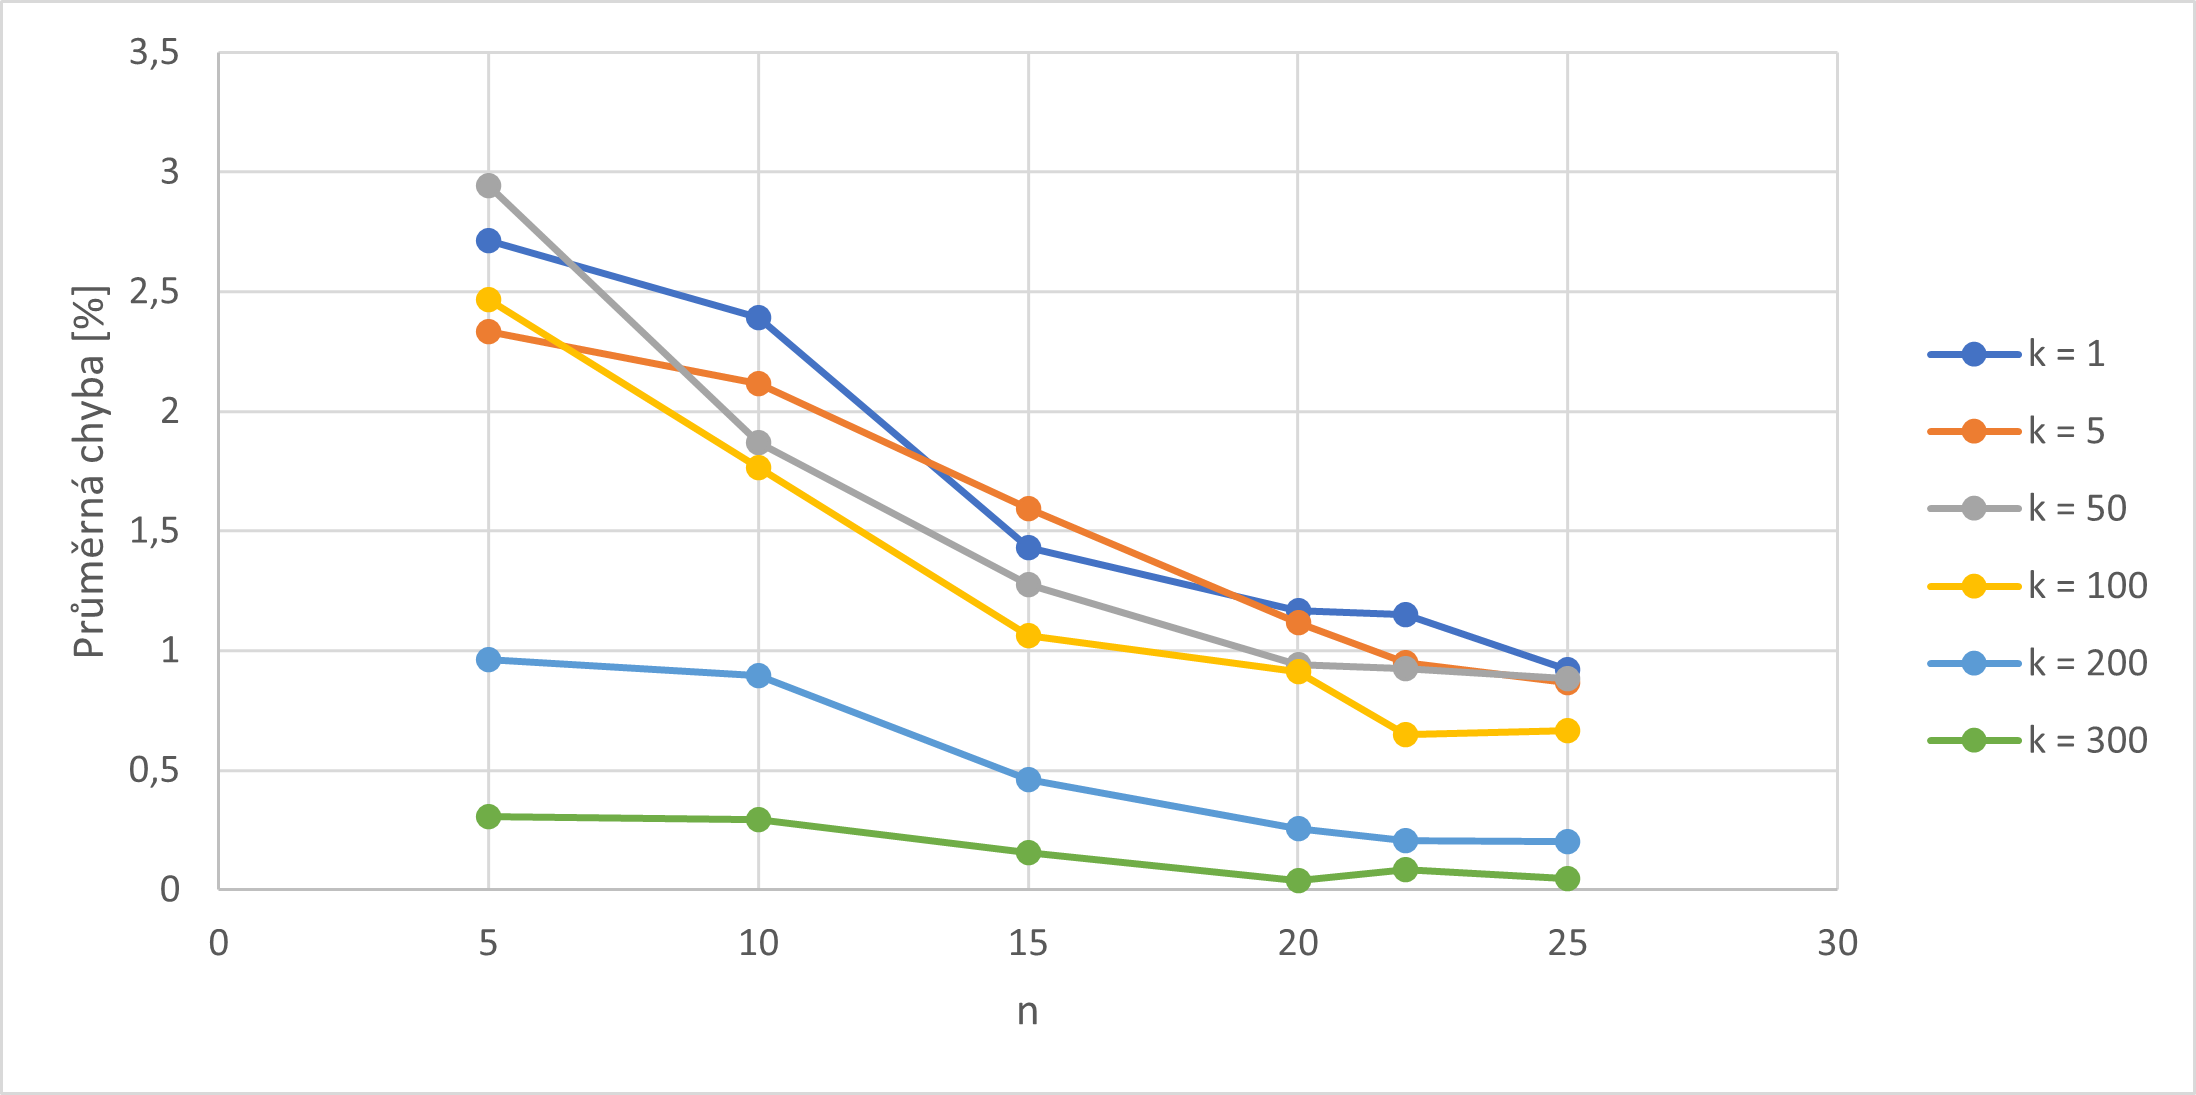
\includegraphics[width=1\textwidth, keepaspectratio]{graphs/greedy/granularity/greedy_granularity_error_n_dep.png}
    \caption{Závislosti průměrné chyby greedy heuristiky na n pro $k \in \{1, 5, 10, 50, 100, 200, 300\}$}
    \label{fig:greedy_granularity_error_n_dep}
\end{figure}

\begin{figure}[ht]\centering
    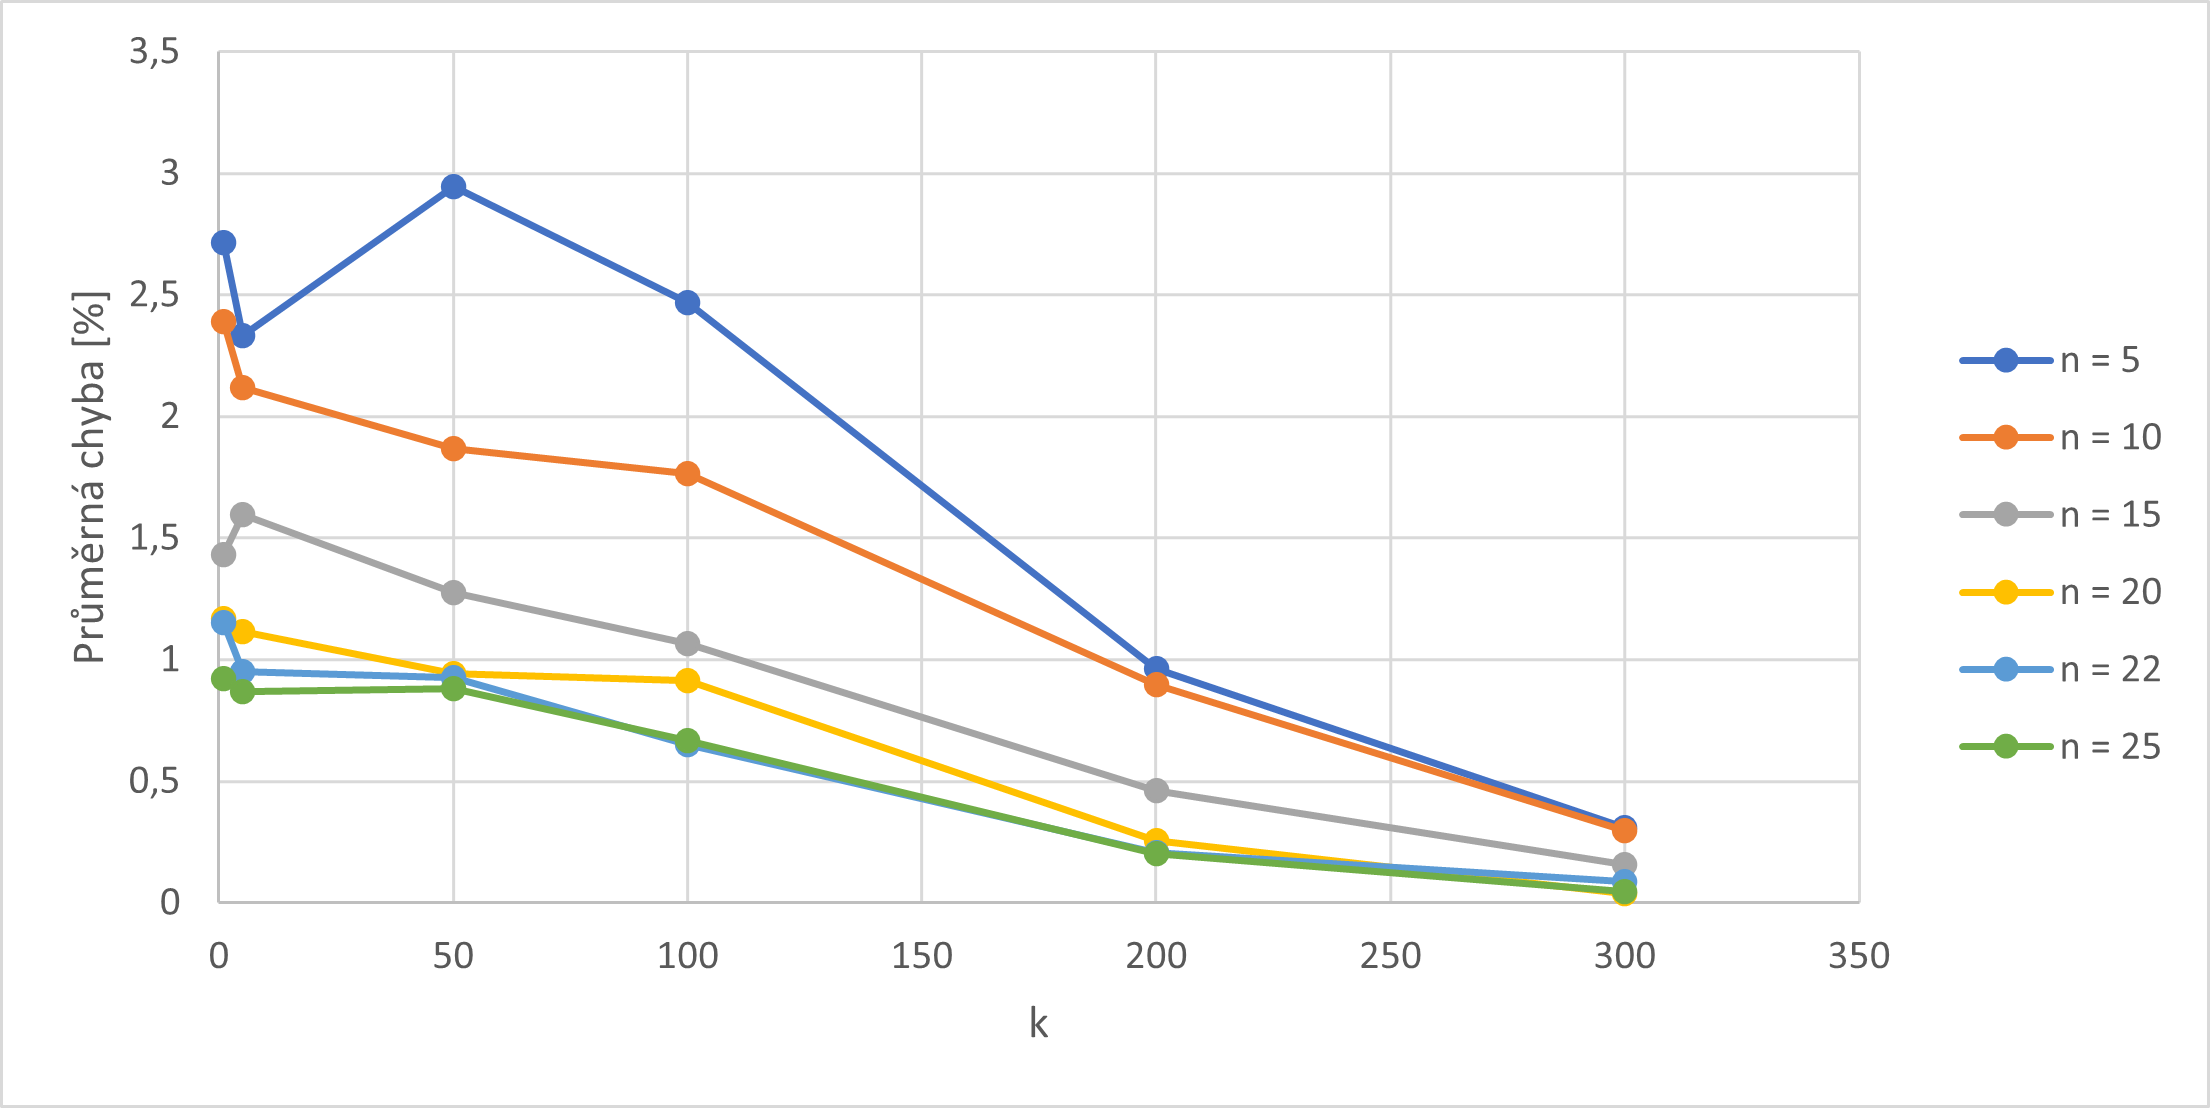
\includegraphics[width=1\textwidth, keepaspectratio]{graphs/greedy/granularity/greedy_granularity_error_k_dep.png}
    \caption{Závislosti průměrné chyby greedy heuristiky na k pro $n \in \{5, 10, 15, 20, 22, 25\}$}
    \label{fig:greedy_granularity_error_k_dep}
\end{figure}

\subsubsection{Citlivost chyby na poměr kapacity batohu k sumární váze}

\subsubsection*{Hypotéza} \label{section:greedy_sum_weight_hyp}

Předpokládejme, že s rostoucím poměrem kapacity batohu vůči sumární váze předmětů bude chybovost heuristiky klesat. Hypotéza je založena na myšlence, že na konci pole předmětů seřazeného dle poměru $\frac{C_i}{m_i}$ zbude méně předmětů tvořících případnou chybu heuristiky.

\subsubsection*{Příprava dat pro experimentální vyhodnocení}

Pro účely experimentálního vyhodnocení byla pro $n \in \{5, 10, 15, 20, 22, 25\}$ vygenerována skupina datových sad s prefixem \textbf{gm}.

Vlastnosti sad (dle konfigurace generátoru) jsou následující:

\begin{center}
    \begin{tabular}{|c | c | c | c | c | c | c|}
        \hline
        -N & -m & -W & -w & -C & -c & -k \\ [0.1ex]
        \hline\hline
        500 & \{0.1 0.2 0.4 0.8 1.0\} & 300 & heavy & 1500 & uni & 1\\
        \hline
    \end{tabular}
\end{center}

\subsubsection*{Výsledky měření}

Naměřené průměrné chyby jsou k dispozici v tabulce \ref{tab:greedy_sum_weight_error}. Chyby byly získány stejně jako v případě \ref{section:greedy_granularity_res}.

Data jsou vizualizována dvěma grafy. Na grafu \ref{fig:greedy_sum_weight_error_n_dep} můžeme pozorovat klesající průměrnou chybu v závislosti na $n$ při rostoucí relativní kapacitě batohu $m$. Výjimku tvoří chyba pro volbu $n=0.5$ a $m=0.5$, kde byla naměřena velmi malá chyba. Na grafu \ref{fig:greedy_granularity_error_k_dep} lze pozorovat klesající průměrnou chybu s rostoucí hodnotou $m$ pro konkrétní volby $n$. Výjimku zde opět tvoří hodnota pro volbu $n=0.5$ a $m=0.5$.

Naměřené výsledky tedy potvrzují hypotézu \ref{section:greedy_sum_weight_hyp}.

\begin{table}
    \begin{center}
         \begin{tabular}{|c | c | c | c | c | c|} 
         \hline
         n & m=0,1 & m=0,2 & m=0,4 & m=0,8 & m=1 \\ [0.1ex] 
         \hline\hline
            5 & 0,127 & 2,897 & 2,991 & 0,317 & 0,000 \\
            \hline
            10 & 5,077 & 3,198 & 1,563 & 0,284 & 0,000 \\
            \hline
            15 & 3,325 & 1,910 & 1,207 & 0,238 & 0,000 \\
            \hline
            20 & 2,767 & 1,748 & 0,999 & 0,211 & 0,000 \\
            \hline
            22 & 2,589 & 1,715 & 0,888 & 0,173 & 0,000 \\
            \hline
            25 & 2,315 & 1,557 & 0,774 & 0,139 & 0,000 \\
            \hline
        \end{tabular}
        \caption{Průměrná chyba greedy heuristiky dle volby m [\%]}
        \label{tab:greedy_sum_weight_error}
    \end{center}
\end{table}

\begin{figure}[ht]\centering
    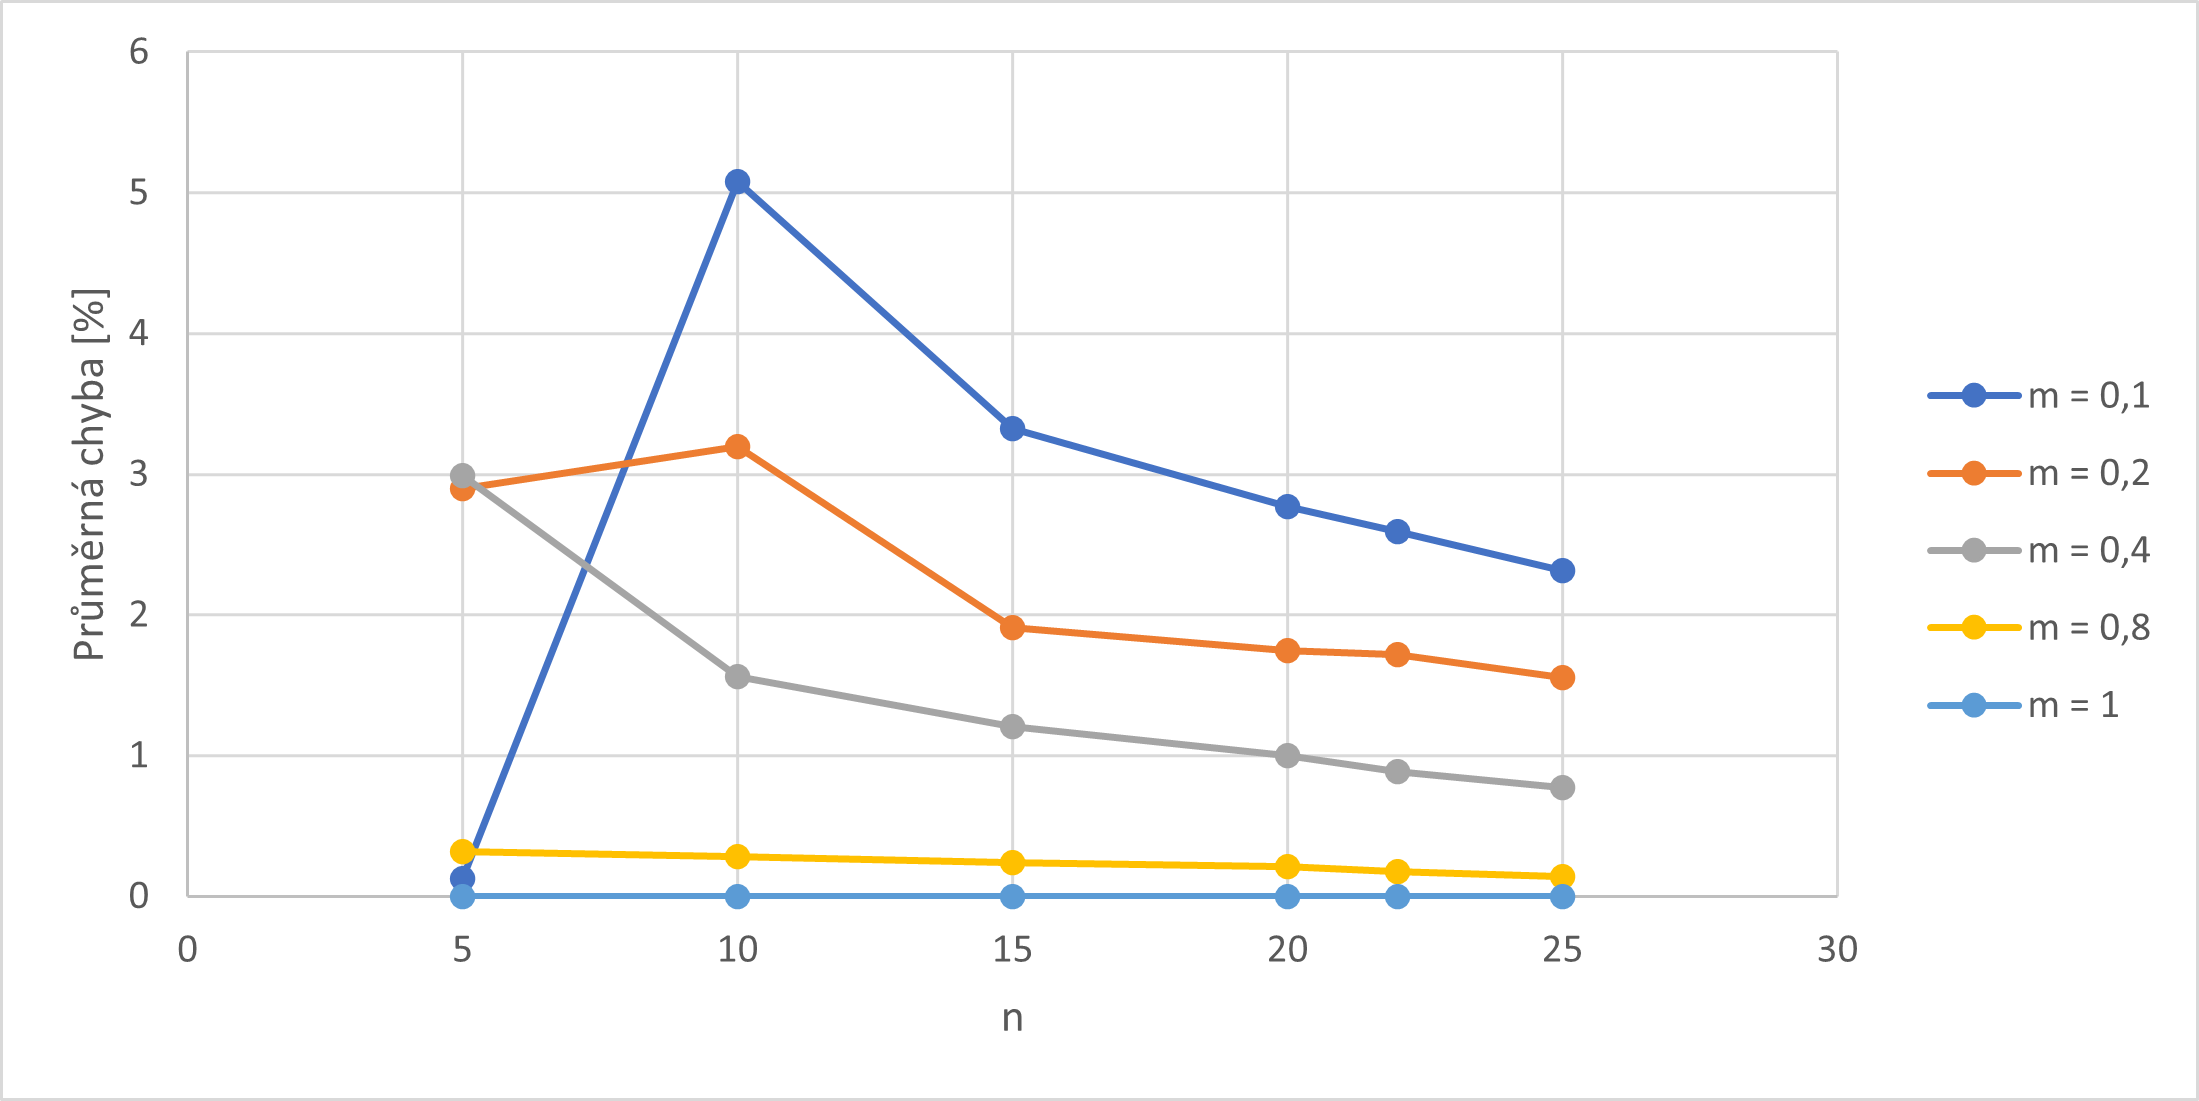
\includegraphics[width=1\textwidth, keepaspectratio]{graphs/greedy/sum_weight/greedy_sum_weight_error_n_dep.png}
    \caption{Závislosti průměrné chyby greedy heuristiky na n pro $m \in \{0.1, 0.2, 0.4, 0.8, 1\}$}
    \label{fig:greedy_sum_weight_error_n_dep}
\end{figure}

\begin{figure}[ht]\centering
    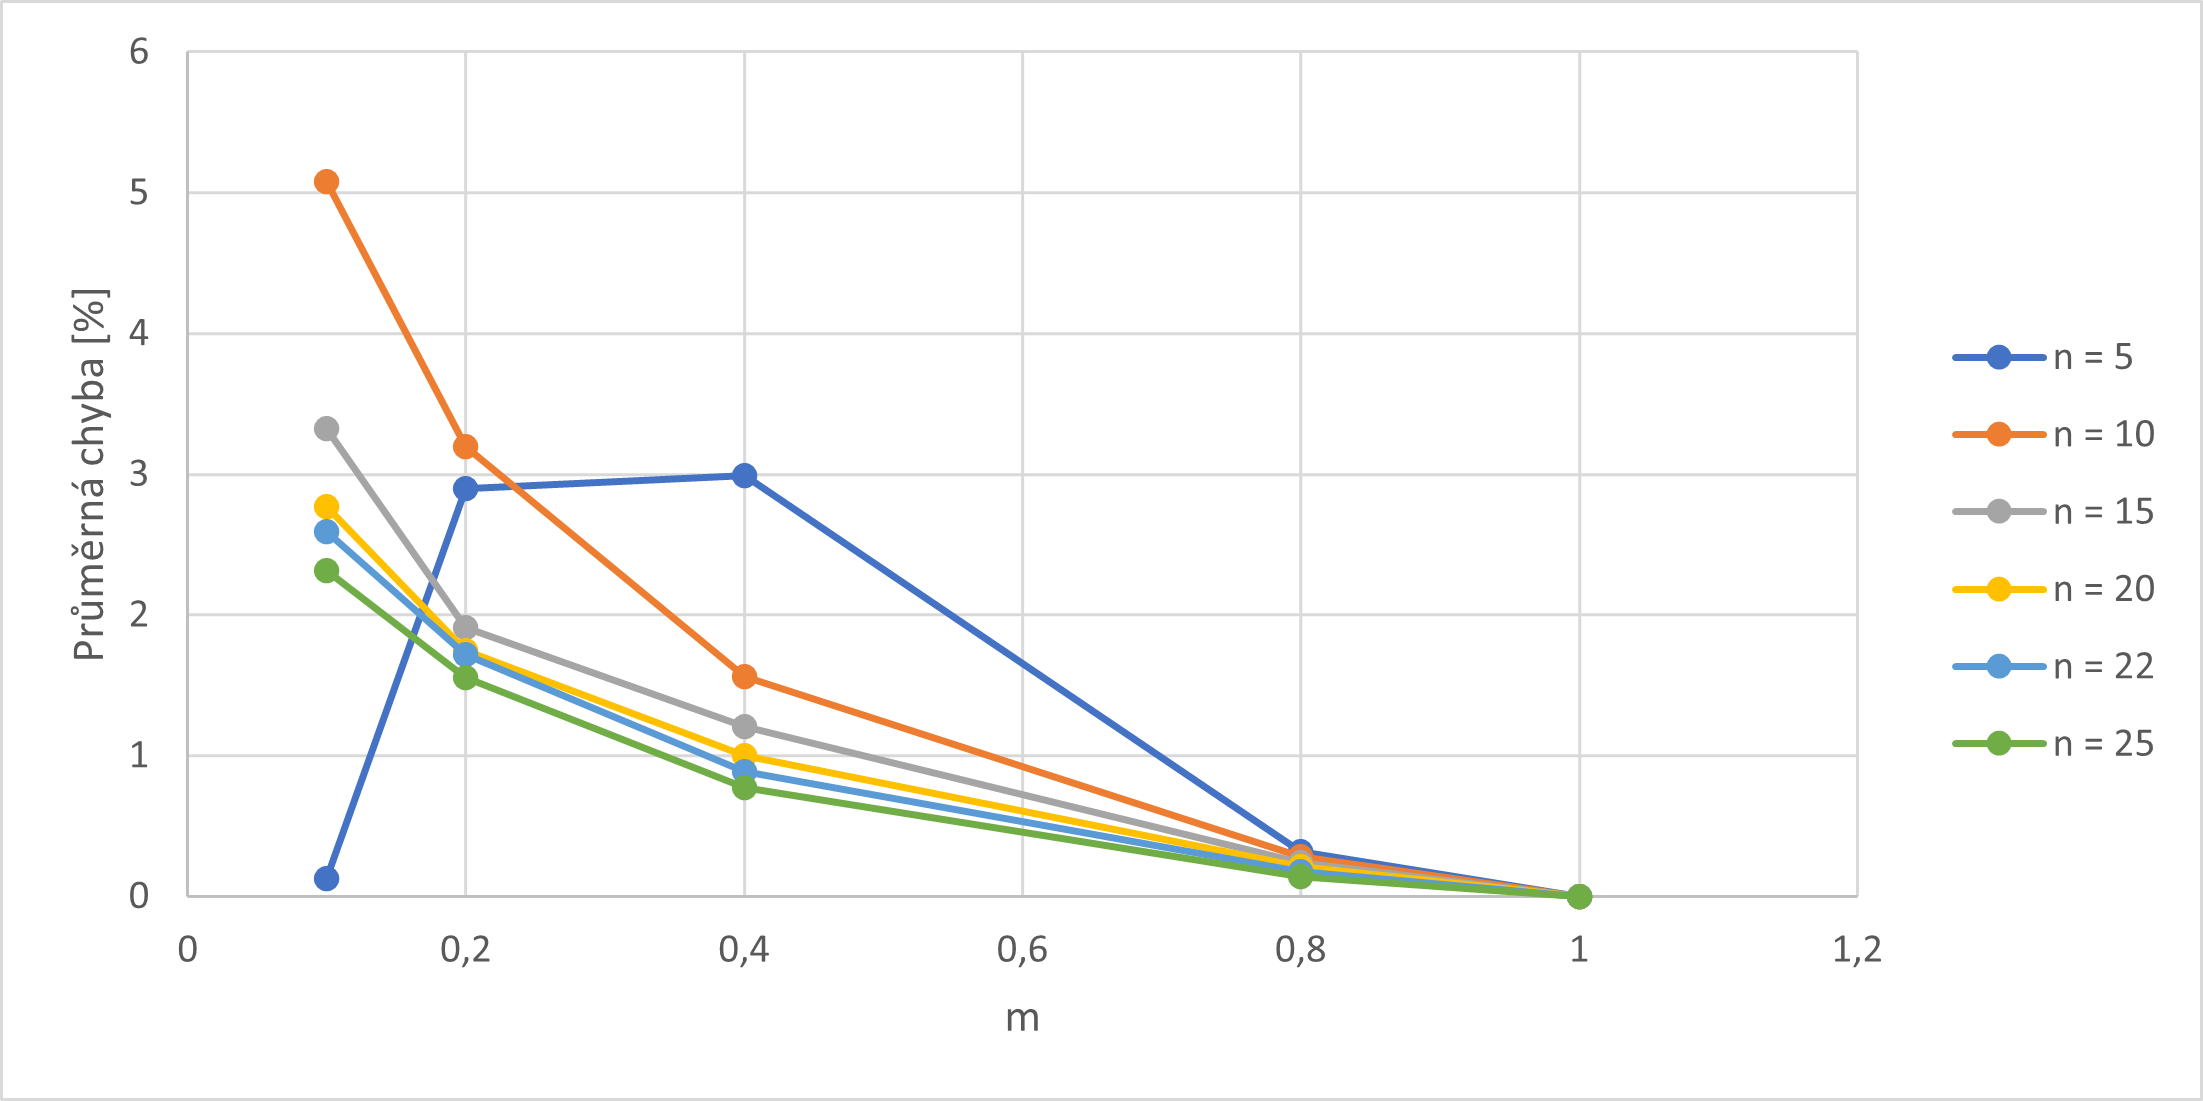
\includegraphics[width=1\textwidth, keepaspectratio]{graphs/greedy/sum_weight/greedy_sum_weight_error_m_dep.png}
    \caption{Závislosti průměrné chyby greedy heuristiky na m pro $n \in \{5, 10, 15, 20, 22, 25\}$}
    \label{fig:greedy_sum_weight_error_m_dep}
\end{figure}

\subsection{Dynamické programování}

\subsubsection{Citlivost výpočetního času na maximální cenu}

\subsubsection*{Hypotéza} \label{section:dp_C_hyp}

Mějme silnou korelaci váhy s cenou. Předpokládejme, že s rostoucí maximální cenou poroste výpočetní čas DP. Hypotéza je založena na skutečnosti, že vyšší maximální cena předmětů povede na vyšší sumární váhu $C_M$, což povede na vyšší složitost, jelikož $C_M$ vystupuje jako činitel v asymptotické složitosti DP při dekompozici dle ceny ($O(n^2 C_M)$).

\subsubsection*{Příprava dat pro experimentální vyhodnocení}

Pro účely experimentálního vyhodnocení byla pro $n \in \{5, 10, 15, 20, 22, 25\}$ vygenerována skupina datových sad s prefixem \textbf{C}.
Vlastnosti sad (dle konfigurace generátoru) jsou následující:

\begin{center}
    \begin{tabular}{|c | c | c | c | c | c | c|}
        \hline
        -N & -m & -W & -w & -C & -c & -k \\ [0.1ex]
        \hline\hline
        500 & 0.8 & 300 & bal & \{100, 500, 1500, 4000\} & strong & 1\\
        \hline
    \end{tabular}
\end{center}

\subsubsection*{Výsledky měření}

Naměřené časy jsou k dispozici v tabulce \ref{tab:dp_C}.

Data jsou vizualizována dvěma grafy. Na grafu \ref{fig:dp_time_n_dep} lze vidět srovnání CPU časů DP v závislosti na n pro konkrétní volby $C$. Můžeme pozorovat růst CPU času s rostoucí hodnotou $C$. Graf \ref{fig:dp_time_C_dep} pak zachycuje závislost CPU času na $C$ pro konkrétní volby $n$. S rostoucí hodnotou $C$ můžeme pozorovat nárůst CPU času potřebného pro vyřešení instance o velikosti $n$.

Naměřené výsledky tedy potvrzují hypotézu \ref{section:dp_C_hyp}.

\begin{table}
    \begin{center}
         \begin{tabular}{|c | c | c | c | c|} 
         \hline
         n & C=100 & C=500 & C=1500 & C=4000 \\ [0.1ex] 
         \hline\hline
            5 & 0,975 & 3,561 & 10,506 & 28,175 \\
            \hline
            10 & 2,749 & 13,396 & 39,599 & 108,353 \\
            \hline
            15 & 6,087 & 29,553 & 87,847 & 242,611 \\
            \hline
            20 & 10,705 & 52,995 & 164,121 & 542,847 \\
            \hline
            22 & 12,861 & 63,961 & 203,433 & 655,499 \\
            \hline
            25 & 16,553 & 83,165 & 302,239 & 858,833 \\
            \hline
        \end{tabular}
        \caption{Průměrný CPU čas DP dle volby C [ms]}
        \label{tab:dp_C}
    \end{center}
\end{table}

\begin{figure}[ht]\centering
    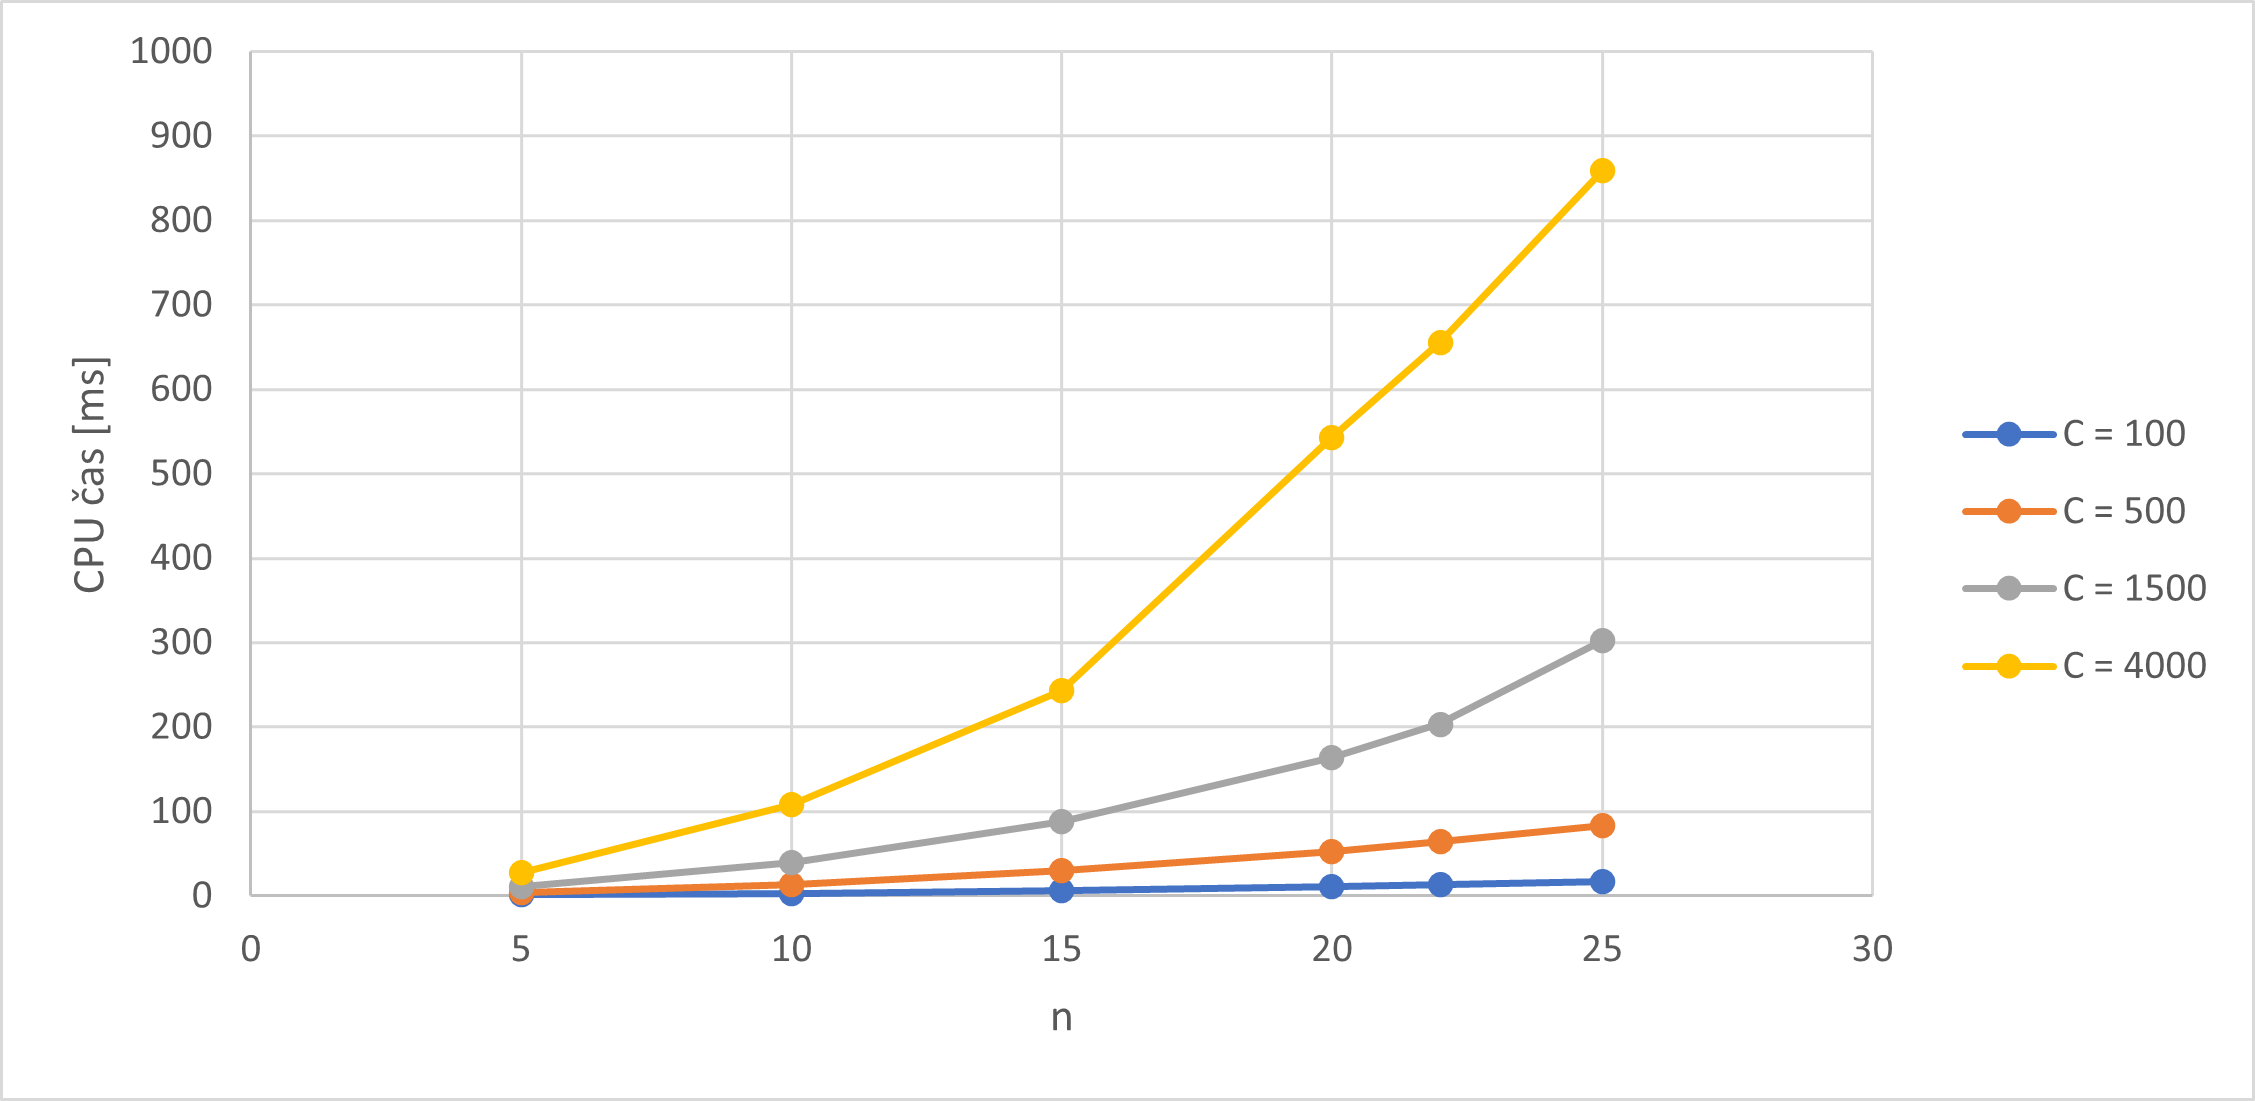
\includegraphics[width=1\textwidth, keepaspectratio]{graphs/dp/dp_time_n_dep.png}
    \caption{Závislosti CPU času DP na n pro $C \in \{100, 500, 1500, 4000\}$}
    \label{fig:dp_time_n_dep}
\end{figure}

\begin{figure}[ht]\centering
    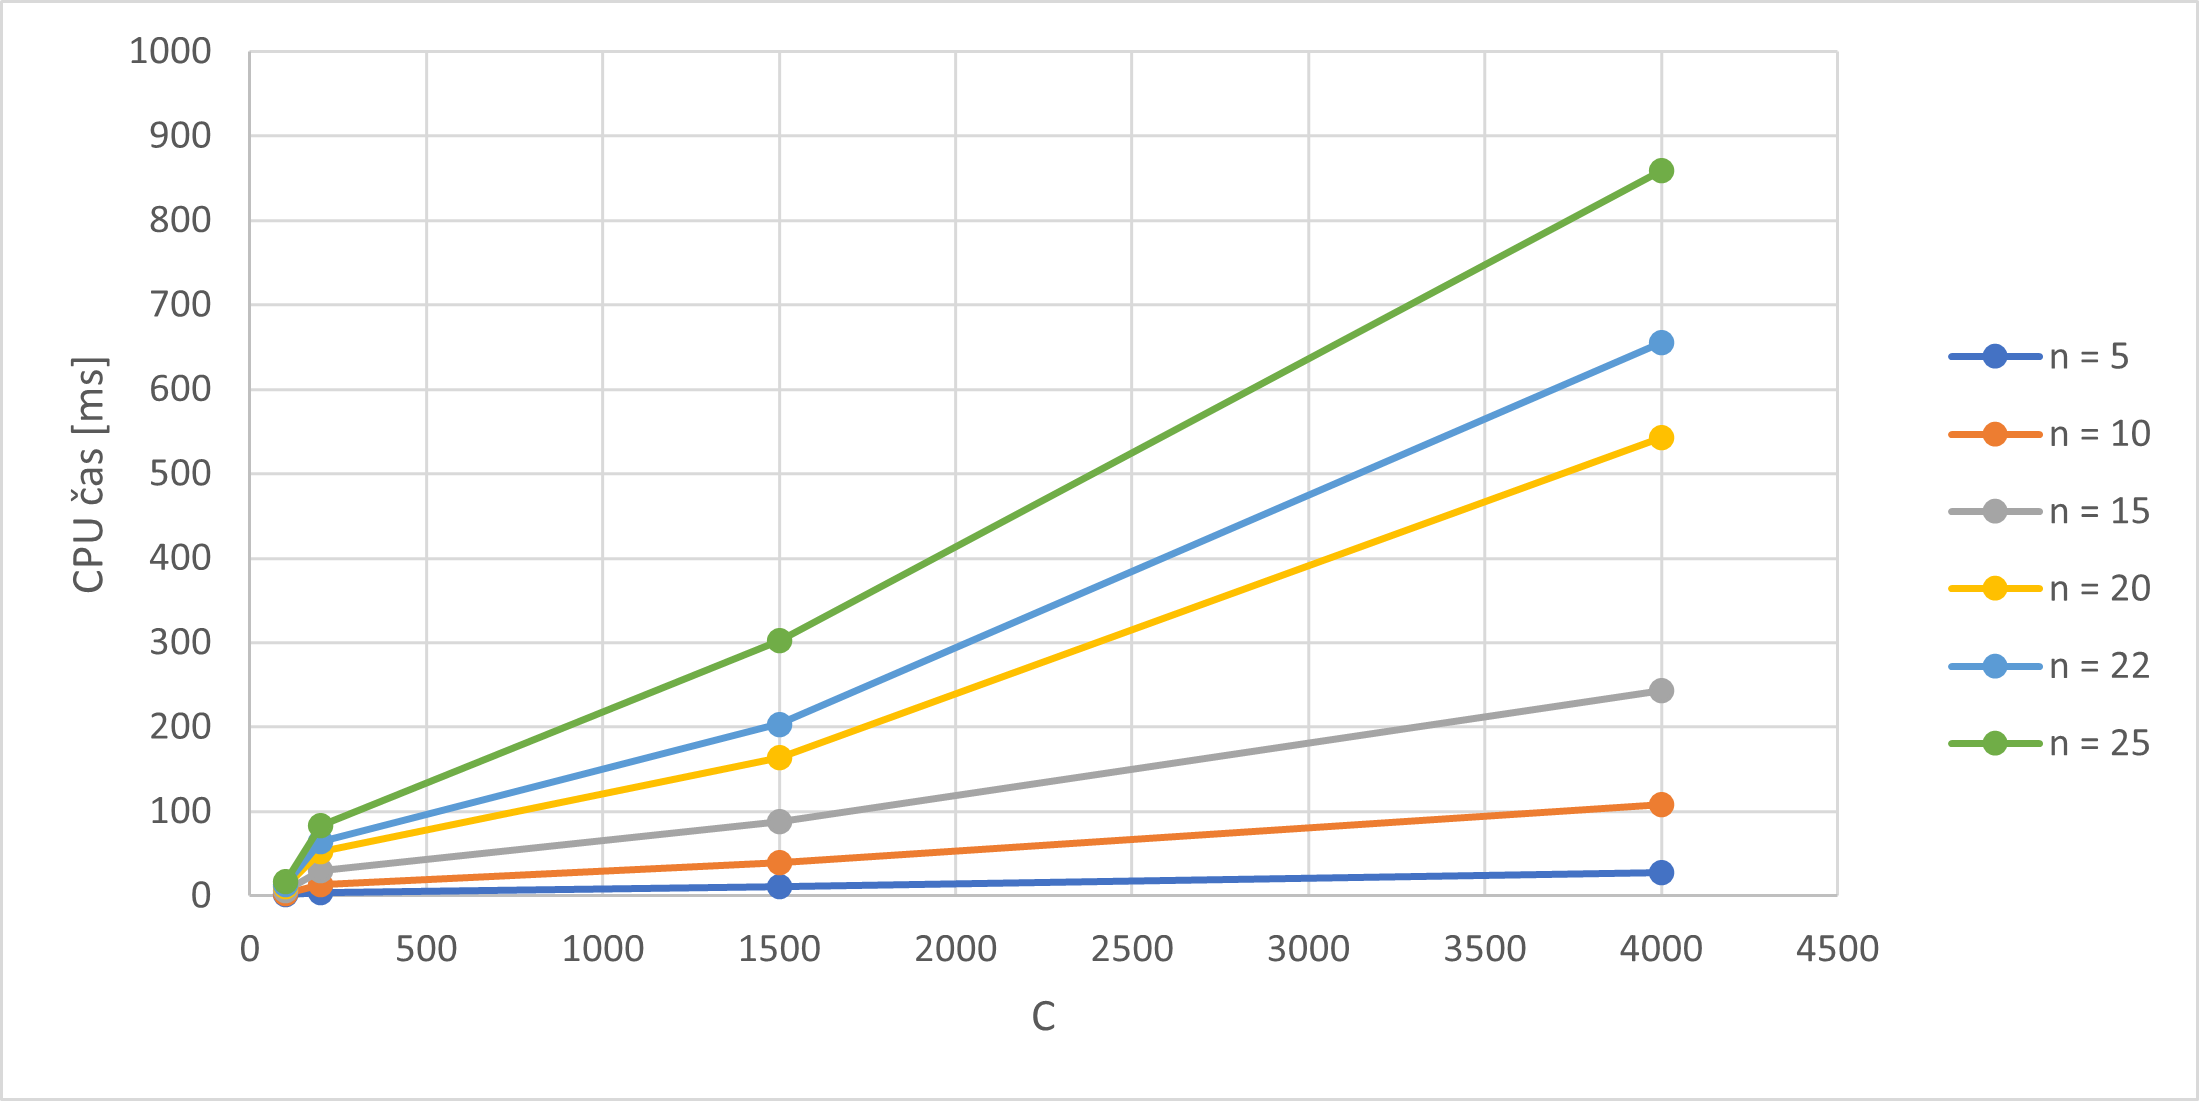
\includegraphics[width=1\textwidth, keepaspectratio]{graphs/dp/dp_time_C_dep.png}
    \caption{Závislosti CPU času DP na C pro $n \in \{5, 10, 15, 20, 22, 25\}$}
    \label{fig:dp_time_C_dep}
\end{figure}

\section{Závěr}

Postupně jsme si uvedli čtyři hypotézy ohledně citlivosti metod řešení na konkrétních vlastnostech sad instancí problémů batohu.

Pro tyto hypotézy jsme připravili příslušné datové sady, nad nimiž jsme experimentálně prozkoumali citlivost příslušných metod prostřednictvím měření.

V případně zkoumání citlivosti času řešení byly zkoumány CPU časy získané zprůměrováním časů ze tří běhů měření. V případě zkoumání citlivosti chyby řešení pak odchylky získaného řešení od optimálnímu řešení, které byly normalizací dle optimálního řešení převedeny na procentuální hodnoty.

Všechny čtyři hypotézy přitom byly výsledky měření potvrzeny.

\end{document}
